\documentclass[fleqn,10pt]{wlscirep}
\usepackage[utf8]{inputenc}
\usepackage[T1]{fontenc}

% Table with Three Lines
\usepackage{booktabs}
\usepackage{longtable}

% Ensure Floats Stay inside the Section
\usepackage[section]{placeins}

% Julia definition (c) 2014 Jubobs
\usepackage[T1]{fontenc}
\usepackage{beramono}
\usepackage{listings}
\usepackage[usenames,dvipsnames]{xcolor}
\lstdefinelanguage{Julia}%
  {morekeywords={abstract, break, case, catch, const, continue, do, else, elseif, %
      end, export, false, for, function, immutable, import, importall, if, in, %
      macro, module, otherwise, quote, return, switch, true, try, type, typealias, %
      using,while, solve, @constraint, @variable, sum, Model, zeros, readxl, openxl, cat},%
   sensitive=true,%
   % alsoother={$},%
   morecomment=[l]{\#},%
   morecomment=[f][\color{forestgreen(web)}][0]{\#},%
   morestring=[s]{"}{"},%
   morestring=[m]{'}{'},%
}[keywords,comments,strings]%

\usepackage{color}
\definecolor{backcolour}{rgb}{0.95,0.95,0.92}
\definecolor{forestgreen(web)}{rgb}{0.13, 0.55, 0.13}
\lstset{%
    language         = Julia,
    basicstyle       = \ttfamily,
    keywordstyle     = \bfseries\color{blue},
    stringstyle      = \color{magenta},
    commentstyle     = \color{forestgreen(web)},
    showstringspaces = false,
    backgroundcolor  = \color{backcolour}, 
    numbers          = left,                    
    numbersep        = 5pt,
    basicstyle       = \footnotesize
}

% Remove the abstract
\usepackage{abstract}
\renewcommand{\abstractname}{}    % clear the title
\renewcommand{\absnamepos}{empty} % originally center

% Allow environments like 'align' to display in multiple pages
\allowdisplaybreaks

% Bold Symbol
\usepackage{bm}

% Code
\usepackage{listings}

% Scale down the tables to the textwidth
\usepackage{graphicx}

% ------------------------------------------------------------
% ------------------------------------------------------------
% ------------------------------------------------------------
\begin{document}

\flushbottom
{\noindent \LARGE \textbf{NonlinearOptim-Assign}} \\
\\[-1em]
{\noindent \textbf{Edward J. Xu (Jie Xu, s181238), edxu96@outlook.com}} \\
\\[-1em]
{\noindent \textbf{DTU Management, Denmark}} \\
\\[-1em]
{\noindent \textbf{Oct 13th, 2019}}

% ------------------------------------------------------------
% ------------------------------------------------------------
% ------------------------------------------------------------

\section{Part A: Method of Lagrange Multipliers}

The decision variables in the problem are summarized in the following table.

\begin{table}[ht]
    \centering
    \begin{tabular}{C C}
        \hline
        \\[-1em]
        Variables & Definition \\
        \\[-1em]
        \hline
        \\[-1em]
        x_{1} & num of dinner \\
        \\[-1em]
        x_{2} & num of drinks \\
        \\[-1em]
        \hline
    \end{tabular}
    \caption{Features of Variables}
    \label{tab:1}
\end{table}
\FloatBarrier

The problem can be formulated as:
\begin{align} \begin{split}
    \max \quad & 8 \ln{x_{1}} + \ln{x_{2}} \\
    \text{s.t.} \quad & 35 x_{1} + 5 x_{2} \leq 315 \\
    & x_{1}, x_{2} \geq 1 \\
    & x_{1}, x_{2} \in \mathbb{R} \\
\end{split} \end{align} 

There exists an optimal solution according to Weierstrass theorem, because The function is continuous, and coercive for maximization (check that objective function increases monotonically when $x_{1}$ or $x_{2}$ increase and there are constraints). Besides, the less equation sign can be replaced by equal sign.

According to the method of Lagrange multipliers, the Lagrangian function of the above problem is:
\begin{align} \begin{split}
    L(x_{1}, x_{2}, \lambda) = 8 \ln{x_{1}} + \ln{x_{2}} - \lambda (35 x_{1} + 5 x_{2} - 315)
\end{split} \end{align} 
which can be maximized by critical points from the following equations:
\begin{align} \begin{split}
    \frac{\partial L}{\partial x_{1}} &= 8 / x_{1} - 35 \lambda = 0 \\
    \frac{\partial L}{\partial x_{2}} &= 1 / x_{2} - 5 \lambda = 0 \\
    \frac{\partial L}{\partial \lambda} &= 35 x_{1} + 5 x_{2} - 315 = 0
\end{split} \end{align} 

By eliminating $\lambda$, we get:
\begin{align} \begin{split}
    x_{1} &= 8 \\
    x_{2} &= 7 \\
    \lambda &= - 1 / 35
\end{split} \end{align} 

So, to have 8 dinners and 7 drinks using 315 euros can maximize the utility.

\section{Part B}

The integrality regrading the bottles is neglected in this part. The decision variabls in the problem are summarized in the following table.

\begin{table}[ht]
    \centering
    \begin{tabular}{C C}
        \hline
        \\[-1em]
        Variables & Definition \\
        \\[-1em]
        \hline
        \\[-1em]
        x_{1} & hours spent producing IPA \\
        \\[-1em]
        x_{2} & hours spent producing Lager \\
        \\[-1em]
        \hline
    \end{tabular}
    \caption{Features of Variables}
    \label{tab:1}
\end{table}
\FloatBarrier

\subsection{Part B 1}

The problem can be formulated as:
\begin{align} \begin{split}
    \max \quad & 15 \sqrt{x_{1}} + 16 \sqrt{x_{2}} \\
    \text{s.t.} \quad & x_{1} + x_{2} \leq 120 \\
    & x_{1}, x_{2} \geq 0
\end{split} \end{align} 

There exists an optimal solution according to Weierstrass theorem, because The function is continuous, and coercive for maximization (check that objective function increases monotonically when $x_{1}$ or $x_{2}$ increase and there are constraints). Besides, the less equation sign can be replaced by equal sign.

The constraint, $x_{1}, x_{2} \geq 0$, is neglected for the time being. According to the method of Lagrange multipliers, the Lagrangian function of the above problem is:
\begin{align} \begin{split}
    L(x_{1}, x_{2}, \lambda) = 15 \sqrt{x_{1}} + 16 \sqrt{x_{2}} - \lambda (x_{1} + x_{2} - 120)
\end{split} \end{align} 
which can be maximized by critical points from the following equations:
\begin{align} \begin{split}
    \frac{\partial L}{\partial x_{1}} &= 15 / 2 \sqrt{x_{1}} - \lambda = 0 \\
    \frac{\partial L}{\partial x_{2}} &= 8 / \sqrt{x_{2}} - \lambda = 0 \\
    \frac{\partial L}{\partial \lambda} &= x_{1} + x_{2} - 120 = 0
\end{split} \end{align} 

By eliminating $\lambda$, we get:
\begin{align} \begin{split}
    x_{1} &= 56.133 \quad \text{so that  } 3 \sqrt{x_{1}} \approx 22.5 \\
    x_{2} &= 63.867 \quad \text{so that  } 4 \sqrt{x_{2}} \approx 32 \\
    \lambda &\approx 1 \\
    15 \sqrt{x_{1}} + 16 \sqrt{x_{2}} &= 240.250 \\
\end{split} \end{align} 
which respects the constraint, $x_{1}, x_{2} \geq 0$.

So I would allocate 56.133 hours in total to produce 22 and half bottles of IPA, and 63.867 hours in total to produce 32 bottles of Lager. The obtained maximum revenue is 240.250.

\subsection{Part B 2}

The problem can be formulated as:
\begin{align} \begin{split}
    \max \quad & 6 \ln{3 \sqrt{x_{1}}} + 4 \ln{4 \sqrt{x_{2}}} \\
    \text{s.t.} \quad & x_{1} + x_{2} \leq 120 \\
    & x_{1}, x_{2} \geq 0
\end{split} \end{align} 

There exists an optimal solution according to Weierstrass theorem, because The function is continuous, and coercive for maximization (check that objective function increases monotonically when $x_{1}$ or $x_{2}$ increase and there are constraints). Besides, the less equation sign can be replaced by equal sign.

The constraint, $x_{1}, x_{2} \geq 0$, is neglected for the time being. According to the method of Lagrange multipliers, the Lagrangian function of the above problem is:
\begin{align} \begin{split}
    L(x_{1}, x_{2}, \lambda) = 6 \ln{3 \sqrt{x_{1}}} + 4 \ln{4 \sqrt{x_{2}}} - \lambda (x_{1} + x_{2} - 120)
\end{split} \end{align} 
which can be maximized by critical points from the following equations:
\begin{align} \begin{split}
    \frac{\partial L}{\partial x_{1}} &= 3 / x_{1} - \lambda = 0 \\
    \frac{\partial L}{\partial x_{2}} &= 2 / x_{2} - \lambda = 0 \\
    \frac{\partial L}{\partial \lambda} &= x_{1} + x_{2} - 120 = 0
\end{split} \end{align} 

By eliminating $\lambda$, we get:
\begin{align} \begin{split}
    x_{1} &= 72 \quad \text{so that  } 3 \sqrt{x_{1}} = 25.45 \\
    x_{2} &= 48 \quad \text{so that  } 4 \sqrt{x_{2}} = 27.71 \\
    \lambda &= 0.042 \\
    6 \ln{3 \sqrt{x_{1}}} + 4 \ln{4 \sqrt{x_{2}}} = 32.709
\end{split} \end{align} 
which respects the constraint, $x_{1}, x_{2} \geq 0$.

So I would allocate 72 hours in total to produce 25.45 and half bottles of IPA, and 48 hours in total to produce 27.71 bottles of Lager. The obtained maximum utility is 32.709.

\subsection{Part B 3: Production with Carl}

How many hours would you ask Carl to help you out to maximize total revenue? How would you divide your own time in producing Lager and IPA in this case? The decision variables are summarized again using the following table.

\begin{table}[ht]
    \centering
    \begin{tabular}{C C}
        \hline
        \\[-1em]
        Variables & Definition \\
        \\[-1em]
        \hline
        \\[-1em]
        x_{1} & hours spent producing IPA \\
        \\[-1em]
        x_{2} & hours spent producing Lager \\
        \\[-1em]
        x_{3} & Carl's hours spent producing Lager \\
        \\[-1em]
        \hline
    \end{tabular}
    \caption{Features of Variables}
    \label{tab:1}
\end{table}
\FloatBarrier

The problem can be formulated as:
\begin{align} \begin{split}
    \max \quad & 15 \sqrt{x_{1}} + 16 \sqrt{x_{2}} + 8 \sqrt{x_{3}} \\
    \text{s.t.} \quad & x_{1} + x_{2} + 0.1 x_{3} \leq 115 \quad \text{if  } x_{3} > 0 \\
    & x_{1} + x_{2} \leq 120 \quad \text{if  } x_{3} = 0 \\
    & x_{3} \leq 60 \\
    & x_{1}, x_{2}, x_{3} \geq 0
\end{split} \end{align} 
where there are two convex functional constraints. Furthermore, it can be easily verified that the objective function is convex. Hence, the corollary applies, so any solution that satisfies the KKT conditions will definitely be an optimal solution.

The Lagrangian function of the above problem is:
\begin{align} \begin{split}
    L(x_{1}, x_{2}, x_{3}, u_{1}, u_{2}) = 15 \sqrt{x_{1}} + 16 \sqrt{x_{2}} + 8 \sqrt{x_{3}} - u_{1} (x_{1} + x_{2} + 0.1 x_{3} - 115) - u_{2} (x_{3} - 60)
\end{split} \end{align} 

KKT conditions are listed:
\begin{align} \begin{split}
    15 / 2 / \sqrt{x_{1}} - u_{1} & \leq 0 \\
    x_{1} (15 / 2 / \sqrt{x_{1}} - u_{1}) &= 0 \\
    8 / \sqrt{x_{2}} - u_{1} & \leq 0 \\
    x_{2} (8 / \sqrt{x_{2}} - u_{1}) &= 0 \\
    4 / \sqrt{x_{3}} - 0.1 u_{1} - u_{2} &\leq 0 \\
    x_{3} (4 / \sqrt{x_{3}} - 0.1 u_{1} - u_{2}) &= 0 \\
    x_{1} + x_{2} + 0.1 x_{3} - 115 &\leq 0 \\
    u_{1} (x_{1} + x_{2} + 0.1 x_{3} - 115) &= 0 \\
    x_{3} - 60 &\leq 0 \\
    u_{2} (x_{3} - 60) &= 0 \\
    x_{1}, x_{2}, x_{3} &\geq 0 \\
    u_{1}, u_{2} &\geq 0
\end{split} \end{align} 

\begin{lstlisting}[language=MATLAB, caption=MATLAB code to solve the equations]
syms x1 x2 x3 u1 u2
eq1 = 15 / 2  - u1 * sqrt(x1) <= 0;
eq2 = x1 * (15 / 2 - u1 * sqrt(x1)) == 0;
eq3 = - u1 * sqrt(x2) + 8 <= 0;
eq4 = x2 * (- u1 * sqrt(x2) + 8) == 0;
eq5 = - 0.1 * u1 * sqrt(x3) - u2 + 4 <= 0;
eq6 = x3 * (- 0.1 * u1 * sqrt(x3) - u2 + 4) == 0;
eq7 = x1 + x2 + 0.1 * x3 - 115 <= 0;
eq8 = u1 * (x1 + x2 + 0.1 * x3 - 115) == 0;
eq9 = x3 - 60 <= 0;
eq10 = u2 * (x3 - 60) == 0;
eq11 = x1 >= 0;
eq12 = x2 >= 0;
eq13 = x3 >= 0;
result = solve([eq1 eq2 eq3 eq4 eq5 eq6 eq7 eq8 eq9 eq10 eq11 eq12 eq13])
\end{lstlisting}

% When $u_{2} = 0$, the conditions becomes:
% \begin{align} \begin{split}
%     15 / 2 / \sqrt{x_{1}} - u_{1} & \leq 0 \\
%     x_{1} (15 / 2 / \sqrt{x_{1}} - u_{1}) &= 0 \\
%     8 / \sqrt{x_{2}} - u_{1} & \leq 0 \\
%     x_{2} (8 / \sqrt{x_{2}} - u_{1}) &= 0 \\
%     4 / \sqrt{x_{3}} - 0.1 u_{1} &\leq 0 \\
%     x_{3} (4 / \sqrt{x_{3}} - 0.1 u_{1}) &= 0 \\
%     x_{1} + x_{2} + 0.1 x_{3} - 115 &\leq 0 \\
%     u_{1} (x_{1} + x_{2} + 0.1 x_{3} - 115) &= 0 \\
%     x_{3} - 60 &\leq 0 \\
%     x_{1}, x_{2}, x_{3} &\geq 0 \\
%     u_{1} &\geq 0
% \end{split} \end{align} 
% where:
% \begin{align} \begin{split}
%     x_{1} &= 56.133 \quad \text{so that  } 3 \sqrt{x_{1}} \approx 22.5 \\
%     x_{2} &= 63.867 \quad \text{so that  } 4 \sqrt{x_{2}} \approx 32 \\
%     \lambda &\approx 1 \\
%     15 \sqrt{x_{1}} + 16 \sqrt{x_{2}} &= 240.250 \\
% \end{split} \end{align} 

% When $x_{3} = 60$, the conditions becomes:
% \begin{align} \begin{split}
%     15 / 2 \sqrt{x_{1}} - u_{1} & \leq 0 \\
%     x_{1} (15 / 2 \sqrt{x_{1}} - u_{1}) &= 0 \\
%     8 / \sqrt{x_{2}} - u_{1} & \leq 0 \\
%     x_{2} (8 / \sqrt{x_{2}} - u_{1}) &= 0 \\
%     4 / \sqrt{60} - 0.1 u_{1} - u_{2} &= 0 \\
%     x_{1} + x_{2} - 109 &\leq 0 \\
%     u_{1} (x_{1} + x_{2} - 109) &= 0 \\
%     x_{1}, x_{2} &\geq 0 \\
%     u_{1}, u_{2} &\geq 0
% \end{split} \end{align} 
% where we get:
% \begin{align} \begin{split}
%     x_{1} = 50.987 \\
%     x_{2} = 58.012 \\
%     u_{1} = 1.050 \\
%     u_{2} = 0.411 \\
%     15 \sqrt{x_{1}} + 16 \sqrt{x_{2}} + 8 \sqrt{x_{3}} = 290.940
% \end{split} \end{align} 

\begin{align} \begin{split}
    x_{1} = 50.987 \\
    x_{2} = 58.012 \\
    x_{3} = 60.000 \\
    u_{1} = 1.050 \\
    u_{2} = 0.411 \\
    15 \sqrt{x_{1}} + 16 \sqrt{x_{2}} + 8 \sqrt{x_{3}} = 290.940
\end{split} \end{align} 

So I would ask Carl to work for 60 hours in total. My time is divided to three parts, of which 50.987 to produce IPA, 58.012 to produce Lager, 5 hours to train Carl, and 6.001 hours to supervise him.

\subsection{Part B 4}

What is the maximum amount you can offer Carl for his services, where you would obtain the same revenue for yourself as without his help (part 1), ignoring production costs?

The problem can be formulated as:
\begin{align} \begin{split}
    \max \quad & - x_{3} \\
    \text{s.t.} \quad & x_{1} + x_{2} + 0.1 x_{3} \leq 115 \\
    & -(15 \sqrt{x_{1}} + 16 \sqrt{x_{2}} + 8 \sqrt{x_{3}}) \leq - 240.250 \\
    & x_{3} \leq 60 \\
    & x_{1}, x_{2}, x_{3} \geq 0
\end{split} \end{align} 
where there are two convex functional constraints. Furthermore, it can be easily verified that the objective function is convex. Hence, the corollary applies, so any solution that satisfies the KKT conditions will definitely be an optimal solution.

The Lagrangian function of the above problem is:
\begin{align} \begin{split}
    L(x_{1}, x_{2}, x_{3}, u_{1}, u_{2}, u_{3}) = - x_{3} - u_{1} (x_{1} + x_{2} + 0.1 x_{3} - 115) - u_{2} (x_{3} - 60) - u_{3}(- 15 \sqrt{x_{1}} - 16 \sqrt{x_{2}} - 8 \sqrt{x_{3}} + 240.250) 
\end{split} \end{align} 

KKT conditions:
\begin{align} \begin{split}
    - u_{1} + 15 u_{3} / 2 / \sqrt{x_{1}} & \leq 0 \\
    x_{1} (- u_{1} + 15 u_{3} / 2 / \sqrt{x_{1}}) & = 0 \\
    - u_{1} + 8 u_{3} / \sqrt{x_{2}} & \leq 0 \\
    x_{2} (- u_{1} + 8 u_{3} / \sqrt{x_{2}}) & = 0 \\
    - 1 - 0.1 u_{1} - u_{2} + 4 u_{3} / \sqrt{x_{3}} & \leq 0 \\
    x_{3} (- 1 - 0.1 u_{1} - u_{2} + 4 u_{3} / \sqrt{x_{3}}) & = 0 \\
    x_{1} + x_{2} + 0.1 x_{3} - 115 & \leq 0 \\
    u_{1} (x_{1} + x_{2} + 0.1 x_{3} - 115) & = 0 \\
    x_{3} - 60 &\leq 0 \\
    u_{2} (x_{3} - 60) &= 0 \\
    15 \sqrt{x_{1}} + 16 \sqrt{x_{2}} + 8 \sqrt{x_{3}} - 240.250 & \geq 0 \\
    u_{3} (15 \sqrt{x_{1}} + 16 \sqrt{x_{2}} + 8 \sqrt{x_{3}} - 240.250) & = 0 \\
    x_{1}, x_{2}, x_{3} &\geq 0 \\
    u_{1}, u_{2}, u_{3} &\geq 0
\end{split} \end{align} 

\begin{lstlisting}[language=MATLAB, caption=MATLAB code to solve the equations]
syms x1 x2 x3 u1 u2 u3
eq1 = - u1 * sqrt(x1) + 15 / 2 * u3 <= 0;
eq2 = x1 * (- u1 * sqrt(x1) + 15 / 2 * u3) == 0;
eq3 = - u1 * sqrt(x2) + 8 * u3 <= 0;
eq4 = x2 * (- u1 * sqrt(x2) + 8 * u3) == 0;
eq5 = - sqrt(x3) - 0.1 * u1 * sqrt(x3) - u2 * sqrt(x3) + 4 * u3 <= 0;
eq6 = x3 * (- sqrt(x3) - 0.1 * u1 * sqrt(x3) - u2 * sqrt(x3) + 4 * u3) == 0;
eq7 = x1 + x2 + 0.1 * x3 - 115 <= 0;
eq8 = u1 * (x1 + x2 + 0.1 * x3 - 115) == 0;
eq9 = x3 - 60 <= 0;
eq10 = u2 * (x3 - 60) == 0;
eq11 = 15 * sqrt(x1) + 16 * sqrt(x2) + 8 * sqrt(x3) - 240.25 >= 0;
eq12 = u3 * (15 * sqrt(x1) + 16 * sqrt(x2) + 8 * sqrt(x3) - 240.25) == 0;
eq13 = x1 >= 0;
eq14 = x2 >= 0;
eq15 = x3 >= 0;
eq16 = u1 >= 0;
eq17 = u2 >= 0;
eq18 = u3 >= 0;
result = solve([eq1 eq2 eq3 eq4 eq5 eq6 eq7 eq8 eq9 eq10 eq11 eq12 eq13 eq14 eq15])
\end{lstlisting}

\section{Part C: Method of Lagrange Multipliers}

\subsection{Part C 1}

The problem can be formulated as:
\begin{align} \begin{split}
    \min \quad & 100 x_{1}^2 + 25 x_{2}^2 + 150 x_{1} x_{2} + 599 x_{3}^2 + 200 x_{2} x_{3} \\
    \text{s.t.} \quad & 0.02 x_{1} + 0.02 x_{2} + 0.05 x_{3} \geq 0.03 \\
    & x_{1} + x_{2} + x_{3} = 1 \\
    & x_{1}, x_{2}, x_{3} \geq 0
\end{split} \end{align} 

According to the method of Lagrange multipliers, the Lagrangian function, $L((x_{1}, x_{2}, x_{3}, \lambda_{1}, \lambda_{2}))$, of the above problem is:
\begin{align} \begin{split}
    L = 100 x_{1}^2 + 25 x_{2}^2 + 150 x_{1} x_{2} + 599 x_{3}^2 + 200 x_{2} x_{3} - \lambda_{1} (0.02 x_{1} + 0.02 x_{2} + 0.05 x_{3} - 0.03) - \lambda_{2} (x_{1} + x_{2} + x_{3} - 1)
\end{split} \end{align} 
which can be minimized by critical points from the following equations:
\begin{align} \begin{split}
    \frac{\partial L}{\partial x_{1}} &= 200 x_{1} + 150 x_{2} - 0.02 \lambda_{1} - \lambda_{2} = 0 \\
    \frac{\partial L}{\partial x_{2}} &= 50 x_{2} + 150 x_{1} + 200 x_{3} - 0.02 \lambda_{1} - \lambda_{2} = 0 \\
    \frac{\partial L}{\partial x_{3}} &= 1198 x_{3} + 200 x_{2} - 0.05 \lambda_{1} - \lambda_{2} = 0 \\
    \frac{\partial L}{\partial \lambda_{1}} &= 0.02 x_{1} + 0.02 x_{2} + 0.05 x_{3} - 0.03 = 0 \\
    \frac{\partial L}{\partial \lambda_{2}} &= x_{1} + x_{2} + x_{3} - 1 = 0
\end{split} \end{align} 

The above systems of equations can be solved by the following code.

\begin{lstlisting}[language=MATLAB, caption=MATLAB code to solve the equations]
syms x1 x2 x3 lambda1 lambda2
eq1 = 200 * x1 + 150 * x2 - 0.02 * lambda1 - lambda2 == 0;
eq2 = 50 * x2 + 150 * x1 + 200 * x3 - 0.02 * lambda1 - lambda2 == 0;
eq3 = 1198 * x3 + 200 * x2 - 0.05 * lambda1 - lambda2 == 0;
eq4 = 0.02 * x1 + 0.02 * x2 + 0.05 * x3 -0.03 == 0;
eq5 = x1 + x2 + x3 - 1 == 0;
eq6 = x1 >= 0;
eq7 = x2 >= 0;
eq8 = x3 >= 0;
result = solve([eq1 eq2 eq3 eq4 eq5 eq6 eq7 eq8])
\end{lstlisting}

\begin{align} \begin{split}
    x_{1} &= 0 \\
    x_{2} &= 0.666 \\
    x_{3} &= 0.333 \\
    \lambda_{1} &= 14422.222 \\
    \lambda_{2} &= -188.444 \\
    100 x_{1}^2 + 25 x_{2}^2 + 150 x_{1} x_{2} + 599 x_{3}^2 + 200 x_{2} x_{3} &= 122.111
\end{split} \end{align} 

So the combination is 0\% fund 1, 2/3\% fund 2, and 1/3\% fund 3. The minimum risk is 122.111.

\subsection{Part C 2}

% The problem can be formulated as:
% \begin{align} \begin{split}
%     \min \quad & 100 x_{1}^2 + 25 x_{2}^2 + 150 x_{1} x_{2} + 599 x_{3}^2 + 200 x_{2} x_{3} \\
%     \text{s.t.} \quad & 0.02 x_{1} + 0.02 x_{2} + 0.05 x_{3} \geq 0.03 \\
%     & x_{1} + x_{2} + x_{3} = 1 \\
%     & x_{1} = y_{1,1} - y_{1,2} \\
%     & x_{2} = y_{2,1} - y_{2,2} \\
%     & x_{3} = y_{3,1} - y_{3,2} \\
%     & y_{1,1}, y_{1,2}, y_{2,1}, y_{2,2}, y_{3,1}, y_{3,2} \geq 0
% \end{split} \end{align} 
% can be minimized by critical points from the following equations:
% \begin{align} \begin{split}
%     \frac{\partial L}{\partial y_{1,1}} &= 200 (y_{1,1} - y_{1,2}) + 150 (y_{2,1} - y_{2,2}) - 0.02 \lambda_{1} - \lambda_{2} = 0 \\
%     \frac{\partial L}{\partial y_{1,2}} &= - 200 (y_{1,1} - y_{1,2}) - 150 (y_{2,1} - y_{2,2}) + 0.02 \lambda_{1} + \lambda_{2} = 0 \\
%     \frac{\partial L}{\partial y_{2,1}} &= 50 (y_{2,1} - y_{2,2}) + 150 (y_{1,1} - y_{1,2}) + 200 (y_{3,1} - y_{3,2}) - 0.02 \lambda_{1} - \lambda_{2} = 0 \\ 
%     \frac{\partial L}{\partial y_{2,2}} &= - 50 (y_{2,1} - y_{2,2}) - 150 (y_{1,1} - y_{1,2}) - 200 (y_{3,1} - y_{3,2}) + 0.02 \lambda_{1} + \lambda_{2} = 0 \\ 
%     \frac{\partial L}{\partial y_{3,1}} &= 1198 (y_{3,1} - y_{3,2}) + 200 (y_{2,1} - y_{2,2}) - 0.05 \lambda_{1} - \lambda_{2} = 0 \\
%     \frac{\partial L}{\partial y_{3,2}} &= - 1198 (y_{3,1} - y_{3,2}) - 200 (y_{2,1} - y_{2,2}) + 0.05 \lambda_{1} + \lambda_{2} = 0 \\
%     \frac{\partial L}{\partial \lambda_{1}} &= 0.02 (y_{1,1} - y_{1,2}) + 0.02 (y_{2,1} - y_{2,2}) + 0.05 (y_{3,1} - y_{3,2}) - 0.03 = 0 \\
%     \frac{\partial L}{\partial \lambda_{2}} &= y_{1,1} - y_{1,2} + y_{2,1} - y_{2,2} + y_{3,1} - y_{3,2} - 1 = 0 \\
% \end{split} \end{align} 

% \begin{lstlisting}[language=MATLAB, caption=MATLAB code to solve the equations]
% syms y11 y12 y21 y22 y31 y32 lambda1 lambda2
% eq1 = 200 * (y11 - y12) + 150 * (y21 - y22) - 0.02 * lambda1 - lambda2 == 0
% eq2 = - 200 * (y11 - y12) - 150 * (y21 - y22) + 0.02 * lambda1 + lambda2 == 0 
% eq3 = 50 * (y21 - y22) + 150 * (y11 - y12) + 200 * (y31 - y32) - 0.02 * lambda1 - lambda2 == 0
% eq4 = - 50 * (y21 - y22) - 150 * (y11 - y12) - 200 * (y31 - y32) + 0.02 * lambda1 + lambda2 == 0
% eq5 =  1198 * (y31 - y32) + 200 * (y21 - y22) - 0.05 * lambda1 - lambda2 == 0
% eq6 = - 1198 * (y31 - y32) - 200 * (y21 - y22) + 0.05 * lambda1 + lambda2 == 0
% eq7 = 0.02 * (y11 - y12) + 0.02 * (y21 - y22) + 0.05 * (y31 - y32) - 0.03 == 0
% eq8 = y11 - y12 + y21 - y22 + y31 - y32 - 1 == 0
% result = solve([eq1 eq2 eq3 eq4 eq5 eq6 eq7 eq8])
% \end{lstlisting}

% \begin{align} \begin{split}
%     y_{1,1} &= 0 \\
%     y_{1,2} &= 0 \\
%     y_{2,1} &= 0.666 \\
%     y_{2,2} &= 0 \\
%     y_{3,3} &= 0.333 \\
%     y_{3,2} &= 0 \\
%     \lambda_{1} &= 14422.222 \\
%     \lambda_{2} &= -188.444 \\
%     100 x_{1}^2 + 25 x_{2}^2 + 150 x_{1} x_{2} + 599 x_{3}^2 + 200 x_{2} x_{3} &= 122.111
% \end{split} \end{align} 

The problem can be formulated as:
\begin{align} \begin{split}
    \min \quad & 100 x_{1}^2 + 25 x_{2}^2 + 150 x_{1} x_{2} + 599 x_{3}^2 + 200 x_{2} x_{3} \\
    \text{s.t.} \quad & 0.02 x_{1} + 0.02 x_{2} + 0.05 x_{3} \geq 0.03 \\
    & x_{1} + x_{2} + x_{3} = 1
\end{split} \end{align} 

The above systems of equations can be solved by the following code.

\begin{lstlisting}[language=MATLAB, caption=MATLAB code to solve the equations]
syms x1 x2 x3 lambda1 lambda2
eq1 = 200 * x1 + 150 * x2 - 0.02 * lambda1 - lambda2 == 0;
eq2 = 50 * x2 + 150 * x1 + 200 * x3 - 0.02 * lambda1 - lambda2 == 0;
eq3 = 1198 * x3 + 200 * x2 - 0.05 * lambda1 - lambda2 == 0;
eq4 = 0.02 * x1 + 0.02 * x2 + 0.05 * x3 -0.03 == 0;
eq5 = x1 + x2 + x3 - 1 == 0;
result = solve([eq1 eq2 eq3 eq4 eq5])
\end{lstlisting}

\begin{align} \begin{split}
    x_{1} &= 0 \\
    x_{2} &= 0.666 \\
    x_{3} &= 0.333 \\
    \lambda_{1} &= 14422.222 \\
    \lambda_{2} &= -188.444 \\
    100 x_{1}^2 + 25 x_{2}^2 + 150 x_{1} x_{2} + 599 x_{3}^2 + 200 x_{2} x_{3} &= 122.111
\end{split} \end{align} 

So we will stick to the previous combination even if we are allowed to short the funds, and the risk is the same.

\section{Part D: Linear Programming and Simplex Algorithm}

The decision variables in the problem are summarized in the following table.

\begin{table}[ht]
    \centering
    \begin{tabular}{C C c}
        \hline
        \\[-1em]
        Variables & Definition & is.integer \\
        \\[-1em]
        \hline
        \\[-1em]
        x_{1,1} & My hours on managing forests per year & Y \\
        \\[-1em]
        x_{1,2} & My hours on hunting per year & Y \\
        \\[-1em]
        x_{1,3} & My hours on managing cabin events per year & Y \\
        \\[-1em]
        x_{2,1} & Uncle's hours on managing forests per year & Y \\
        \\[-1em]
        x_{2,2} & Uncle's hours on hunting per year & Y \\
        \\[-1em]
        x_{2,3} & Uncle's hours on managing cabin events per year & Y \\
        \\[-1em]
        x_{3,1} & Cousin's hours on managing forests per year & Y \\
        \\[-1em]
        x_{3,2} & Cousin's hours on hunting per year & Y \\
        \\[-1em]
        x_{3,3} & Cousin's hours on managing cabin events per year & Y \\
        \\[-1em]
        x_{4} & Num of cabin events per year & Y \\
        \\[-1em]
        \hline
    \end{tabular}
    \caption{Features of Variables}
    \label{tab:1}
\end{table}
\FloatBarrier

The constraints about forest areas are omitted. To be more specific, there is no limit on the number of harvested christmas trees. Then the problem can be formulated as:
\begin{align} \begin{split}
    \max \quad & 1000 (x_{1,1} + x_{2,1} + x_{3,1}) + 750 (x_{1,2} + x_{2,2} + x_{3,2}) + 2000 x_{4} \\
    \text{s.t.} \quad 
    & x_{1,1} + x_{1,2} + x_{1,3} \leq 40 \\
    & x_{2,1} + x_{2,2} + x_{2,3} \leq 50 \\
    & x_{3,1} + x_{3,2} + x_{3,3} \leq 60 \\
    & x_{1,1} \geq 20 \\
    & x_{2,1} = 0 \\
    & x_{2,2} \geq 20 \\
    & x_{2,3} \leq 50 / 3 \\
    & x_{3,3} \geq 3 (x_{1,3} + x_{2,3}) \\
    & x_{1,2} + x_{2,2} + x_{3,2} \leq 30 \\
    & x_{4} \leq 20 \\
    & x_{1,3} + x_{2,3} + x_{3,3} \geq 2 x_{4} \\
    & x_{1,1}, x_{1,2}, x_{1,3}, x_{2,1}, x_{2,2}, x_{2,3}, x_{3,1}, x_{3,2}, x_{3,3}, x_{4} \in \mathbb{Z}^{+}
\end{split} \end{align} 

\subsection{Problem D2: Simplex Algorithm}

Write the problem in standard form:
\begin{align} \begin{split}
    \max \quad & 1000 (x_{1,1} + x_{2,1} + x_{3,1}) + 750 (x_{1,2} + x_{2,2} + x_{3,2}) + 2000 x_{4} \\
    \text{s.t.} \quad 
    & x_{1,1} + x_{1,2} + x_{1,3} \leq 40 \\
    & x_{2,1} + x_{2,2} + x_{2,3} \leq 50 \\
    & x_{3,1} + x_{3,2} + x_{3,3} \leq 60 \\
    & - x_{1,1} \leq - 20 \\
    & x_{2,1} = 0 \\
    & - x_{2,2} \leq - 20 \\
    & x_{2,3} \leq 50 / 3 \\
    & - x_{3,3} + 3 x_{1,3} + 3 x_{2,3} \leq 0 \\
    & x_{1,2} + x_{2,2} + x_{3,2} \leq 30 \\
    & x_{4} \leq 20 \\
    & - x_{1,3} - x_{2,3} - x_{3,3} + 2 x_{4} \leq 0 \\
    & x_{1,1}, x_{1,2}, x_{1,3}, x_{2,1}, x_{2,2}, x_{2,3}, x_{3,1}, x_{3,2}, x_{3,3}, x_{4} \in \mathbb{Z}^{+}
\end{split} \end{align} 

\begin{table} % [ht]
    \centering
    \resizebox{\textwidth}{!}{
        \begin{tabular}{ccccccccccccccccccccccc}
            \hline
            \\[-1em]
            BV & Z & x_{1,1} & x_{1,2} & x_{1,3} & x_{2,1} & x_{2,2} & x_{2,3} & x_{3,1} & x_{3,2} & x_{3,3} & x_{4} & y_{1} & y_{2} & y_{3} & y_{4} & y_{5} & y_{6} & y_{7} & y_{8} & y_{9} & y_{10} & b \\
            \\[-1em]
            \hline
            \\[-1em]
            Z & 1 & -1000 & -750 & 0 & -1000 & -750 & 0 & -1000 & -750 & 0 & -2000 & 0 & 0 & 0 & 0 & 0 & 0 & 0 & 0 & 0 & 0 & 0 \\
            \\[-1em]
            $y_{1}$ & 0 & 1 & 1 & 1 & 0 & 0 & 0 & 0 & 0 & 0 & 0 & 1 & 0 & 0 & 0 & 0 & 0 & 0 & 0 & 0 & 0 & 40 \\
            \\[-1em]
            $y_{2}$ & 0 & 0 & 0 & 0 & 1 & 1 & 1 & 0 & 0 & 0 & 0 & 0 & 1 & 0 & 0 & 0 & 0 & 0 & 0 & 0 & 0 & 50 \\
            \\[-1em]
            $y_{3}$ & 0 & 0 & 0 & 0 & 0 & 0 & 0 & 1 & 1 & 1 & 0 & 0 & 0 & 1 & 0 & 0 & 0 & 0 & 0 & 0 & 0 & 60 \\
            \\[-1em]
            $y_{4}$ & 0 & 1 & 0 & 0 & 0 & 0 & 0 & 0 & 0 & 0 & 0 & 0 & 0 & 0 & 1 & 0 & 0 & 0 & 0 & 0 & 0 & - 20 \\
            \\[-1em]
            $y_{5}$ & 0 & 0 & 0 & 0 & 1 & 0 & 0 & 0 & 0 & 0 & 0 & 0 & 0 & 0 & 0 & 1 & 0 & 0 & 0 & 0 & 0 & 0 \\
            \\[-1em]
            $y_{6}$ & 0 & 0 & 0 & 0 & 0 & -1 & 0 & 0 & 0 & 0 & 0 & 0 & 0 & 0 & 0 & 0 & 1 & 0 & 0 & 0 & 0 & -20 \\
            \\[-1em]
            $y_{7}$ & 0 & 0 & 0 & 0 & 0 & 0 & 1 & 0 & 0 & 0 & 0 & 0 & 0 & 0 & 0 & 0 & 0 & 1 & 0 & 0 & 0 & 50 / 3 \\
            \\[-1em]
            $y_{8}$ & 0 & 0 & 0 & 3 & 0 & 0 & 3 & 0 & 0 & -1 & 0 & 0 & 0 & 0 & 0 & 0 & 0 & 0 & 1 & 0 & 0 & 0 \\
            \\[-1em]
            $y_{9}$ & 0 & 0 & 1 & 0 & 0 & 1 & 0 & 0 & 1 & 0 & 0 & 0 & 0 & 0 & 0 & 0 & 0 & 0 & 0 & 1 & 0 & 30 \\
            \\[-1em]
            $y_{10}$ & 0 & 0 & 0 & 0 & 0 & 0 & 0 & 0 & 0 & 0 & 1 & 0 & 0 & 0 & 0 & 0 & 0 & 0 & 0 & 0 & 1 & 20 \\
            \\[-1em]
            \hline
        \end{tabular}
    }
    \caption{Simplex Algorithm in Tabular Form}
    \label{tab-sa1}
\end{table}
\FloatBarrier

The first iteration of simplex algorithm for solving the above problem is illustrated in table \ref{tab-sa1} and table \ref{tab-sa2}. During the first iteration, $x_{4}$ is selected as the entering basic variable, of which the coefficient has the maximum absolute value in first row. Solve the new BF solution, and update first row.

\begin{table} % [ht]
    \centering
    \resizebox{\textwidth}{!}{
        \begin{tabular}{ccccccccccccccccccccccc}
            \hline
            \\[-1em]
            BV & Z & x_{1,1} & x_{1,2} & x_{1,3} & x_{2,1} & x_{2,2} & x_{2,3} & x_{3,1} & x_{3,2} & x_{3,3} & x_{4} & y_{1} & y_{2} & y_{3} & y_{4} & y_{5} & y_{6} & y_{7} & y_{8} & y_{9} & y_{10} & b \\
            \\[-1em]
            \hline
            \\[-1em]
            Z & 1 & -1000 & -750 & 0 & -1000 & -750 & 0 & -1000 & -750 & 0 & 0 & 0 & 0 & 0 & 0 & 0 & 0 & 0 & 0 & 0 & 2000 & 40000 \\
            \\[-1em]
            $y_{1}$ & 0 & 1 & 1 & 1 & 0 & 0 & 0 & 0 & 0 & 0 & 0 & 1 & 0 & 0 & 0 & 0 & 0 & 0 & 0 & 0 & 0 & 40 \\
            \\[-1em]
            $y_{2}$ & 0 & 0 & 0 & 0 & 1 & 1 & 1 & 0 & 0 & 0 & 0 & 0 & 1 & 0 & 0 & 0 & 0 & 0 & 0 & 0 & 0 & 50 \\
            \\[-1em]
            $y_{3}$ & 0 & 0 & 0 & 0 & 0 & 0 & 0 & 1 & 1 & 1 & 0 & 0 & 0 & 1 & 0 & 0 & 0 & 0 & 0 & 0 & 0 & 60 \\
            \\[-1em]
            $y_{4}$ & 0 & 1 & 0 & 0 & 0 & 0 & 0 & 0 & 0 & 0 & 0 & 0 & 0 & 0 & 1 & 0 & 0 & 0 & 0 & 0 & 0 & - 20 \\
            \\[-1em]
            $y_{5}$ & 0 & 0 & 0 & 0 & 1 & 0 & 0 & 0 & 0 & 0 & 0 & 0 & 0 & 0 & 0 & 1 & 0 & 0 & 0 & 0 & 0 & 0 \\
            \\[-1em]
            $y_{6}$ & 0 & 0 & 0 & 0 & 0 & -1 & 0 & 0 & 0 & 0 & 0 & 0 & 0 & 0 & 0 & 0 & 1 & 0 & 0 & 0 & 0 & -20 \\
            \\[-1em]
            $y_{7}$ & 0 & 0 & 0 & 0 & 0 & 0 & 1 & 0 & 0 & 0 & 0 & 0 & 0 & 0 & 0 & 0 & 0 & 1 & 0 & 0 & 0 & 50 / 3 \\
            \\[-1em]
            $y_{8}$ & 0 & 0 & 0 & 3 & 0 & 0 & 3 & 0 & 0 & -1 & 0 & 0 & 0 & 0 & 0 & 0 & 0 & 0 & 1 & 0 & 0 & 0 \\
            \\[-1em]
            $y_{9}$ & 0 & 0 & 1 & 0 & 0 & 1 & 0 & 0 & 1 & 0 & 0 & 0 & 0 & 0 & 0 & 0 & 0 & 0 & 0 & 1 & 0 & 30 \\
            \\[-1em]
            $x_{4}$ & 0 & 0 & 0 & 0 & 0 & 0 & 0 & 0 & 0 & 0 & 1 & 0 & 0 & 0 & 0 & 0 & 0 & 0 & 0 & 0 & 1 & 20 \\
            \\[-1em]
            \hline
        \end{tabular}
    }
    \caption{Simplex Algorithm in Tabular Form}
    \label{tab-sa2}
\end{table}
\FloatBarrier

\subsection{Part D 3}

The dual problem is:
\begin{align} \begin{split}
    \min \quad & 40 y_{1} + 50 y_{2} + 60 y_{3} + 20 y_{4} + 20 y_{6} + 50 / 3 y_{7} + 30 y_{9} + 20 y_{10} \\
    \text{s.t.} \quad 
    & y_{1} + y_{4} \geq 1000 \\
    & y_{1} + y_{9} \geq 1000 \\
    & y_{1} - 3 y_{8} + y_{11} \geq 1000 \\
    & y_{2} + y_{5} \geq 750 \\
    & y_{2} + y_{6} \geq 750 \\
    & y_{2} + y_{7} - 3 y_{8} + y_{11} \geq 750 \\
    & y_{3} \geq 0 \\
    & y_{3} + y_{9} \geq 0 \\
    & y_{3} + y_{8} + y_{11} \geq 0 \\
    & y_{10} - 2 y_{11} \geq 2000 \\
    & y_{1} + y_{2} + y_{3} + y_{7} + y_{9} + y_{10} \geq 0 \\
    & y_{4} + y_{6} + y_{8} + y_{11} \leq 0 \\
    & y_{5} = 0
\end{split} \end{align} 

\subsection{Part D 4}

Put the solution in all constraints. If all are respected, then it is a feasible solution. Change all the inequality to equality constraints, and find those met by the set. If two or more equality constraints are met, then the solution is one of the cross sections in the edge of the feasible region. Move the solution along the edges to see if there is a better solution. If not, the solution is the optimal one.

\subsection{Part D 5}

There is no sufficient coefficients.

\section{Part E: Linear Programming}

\begin{align} \begin{split}
    \max \quad & 2 x_{1}+3 x_{2} \\
    \text{s.t.} \quad 
    & 2 x_{1} + x_{2} \leq 16 \\ 
    & x_{1} - x_{2} \leq 2 \\
    & -x_{1} + 2 x_{2} \geq 4 \\
    & x_{2} \leq 6 \\ 
    & x_{1}, x_{2} \geq 0 
\end{split} \end{align} 

\begin{figure}[ht]
    \centering
    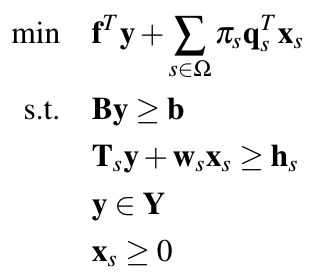
\includegraphics[width=0.6\linewidth]{./images/1.jpg}
    \caption{Illustration of Feasible Regions}
    \label{fig:1}
\end{figure}

So the point (4, 6) is the optimal solution.

If we add the following constraint to the problem, the optimal solution will change. The new optimal solution is (8 / 3, 10 / 3).
\begin{align} \begin{split}
    x_{1} - x_{2} \geq - 6
\end{split} \end{align} 

If the objective function is nonlinear, the optimal soluation may lay on some point in the feasible edges instead of the feasible points. I would compare the value of the points whose slope equals the feasible edges.

\section{Part F: Lagrangian Dual Problem}

\subsection{Part F 1}

\begin{align} \begin{split}
    \max \quad & x_{1}^{2} + 6 x_{2} + 4 x_{3}^{2} \\
    \text{s.t.} \quad & 2 x_{1} + x_{2} + 4 x_{3} \leq 10 \\ 
    & x_{1}, x_{3} \geq 0 \\ 
    & x_{2} \in (0, 1) \\
\end{split} \end{align} 

The Lagrangian dual function is:
\begin{align} \begin{split}
    L(x_{1}, x_{2}, x_{3}, \lambda) = - x_{1}^{2} - 6 x_{2} - 4 x_{3}^{2} + \lambda (- 10 + 2 x_{1} + x_{2} + 4 x_{3} )
\end{split} \end{align} 

\begin{align} \begin{split}
    \theta(\lambda) &= - 10 \lambda + \max\{- x_{1}^{2} + 2 \lambda x_{1} \} + \max\{(\lambda - 6) x_{2} \} + \max\{- 4 x_{3}^{2} + 4 \lambda x_{3} \}
\end{split} \end{align} 

For a fixed value of $\lambda > 0$, the maximum of $L(x_{1}, x_{2}, x_{3}, \lambda)$ over $x \in X$ is attained at:
\begin{align} \begin{split}
    x_{1}(\lambda) &= \lambda \\
    x_{2}(\lambda) &= \begin{cases}
        & 0 \quad \text{when  } \lambda \leq 6 \\
        & 1 \quad \text{when  } \lambda > 6
    \end{cases} \\
    x_{3}(\lambda) &= \lambda / 2
\end{split} \end{align} 

So, we get $L(x_{1}(\lambda), x_{2}(\lambda), x_{3}(\lambda), \lambda)$, when $\lambda \leq 6$:
\begin{align} \begin{split}
    L(x_{1}(\lambda), x_{2}(\lambda), x_{3}(\lambda), \lambda) &= - 10 \lambda + \lambda^2 + \lambda^2 \\
    &= - 10 \lambda + 2 \lambda^2
\end{split} \end{align} 
of which the minimum is $\lambda = 2.5$. Then, $x_{1} = 2.5$, $x_{2} = 0$, $x_{1} = 1.25$, and objective value is 12.5.

While when $\lambda > 6$, it becomes:
\begin{align} \begin{split}
    L(x_{1}(\lambda), x_{2}(\lambda), x_{3}(\lambda), \lambda) &= - 10 \lambda + \lambda^2 + (\lambda - 6) + \lambda^2 \\
    &= 2 \lambda^2 - 9 \lambda - 6
\end{split} \end{align} 
of which the minimum is $\lambda = 2.25$, Then, $x_{1} = 2.25$, $x_{2} = 1$, $x_{1} = 1.125$, and objective value is 10.125.

So the maximum value is 12.5, when $x_{1} = 2.5$, $x_{2} = 0$, $x_{1} = 1.25$.

\subsection{Part F 2}

It can also be solved by using KKT conditions.

\section{Part G: Gradient Search Algorithm}

Illustration two iterations of Gradient Search Algorithm to optimize the following question:
\begin{align} \begin{split}
    \max \quad f(\boldsymbol{x}) = 4 x_{1} + 2 x_{1} x_{2} - x_{2} - 4 x_{1}^{2} - x_{2}^{2}
\end{split} \end{align} 

Thus,
\begin{align} \begin{split}
    \frac{\partial f}{\partial x_{1}} &= 4 + 2 x_{2} - 8 x_{1} \\
    \frac{\partial f}{\partial x_{2}} &= -1 + 2 x_{1} - 2 x_{2} \\
\end{split} \end{align} 

Suppose that $\boldsymbol{x}' = (1, 1)$ as the initial trial solution. Then the gradient is:
\begin{align} \begin{split}
    \nabla f(\boldsymbol{x}') = (- 2, -1)
\end{split} \end{align} 

Substitute $\boldsymbol{x}' + t \nabla f(\boldsymbol{x}')$ in to $f$:
\begin{align} \begin{split}
    f(\boldsymbol{x}' + t \nabla f(\boldsymbol{x}')) &= f(1 - 2t, 1 - t) \\
    &= 4 (1 - 2t) + 2 (1 - 2t) (1 - t) - (1 - t) - 4 (1 - 2t)^{2} - (1 - t)^{2} \\
    &= 5 t - 13 t^2
\end{split} \end{align} 
which can be maximized at $t = 5 / 26$ by the following equations:
\begin{align} \begin{split}
    \frac{\partial (5 t - 13 t^2)}{\partial t} = 5 - 26 t
\end{split} \end{align} 

Reset $\boldsymbol{x}' = (1, 1) + 5 / 26 (-2, -1) = (0.6154, 0.8077)$. Repeat the above procedure again.

Solve $\nabla f(\boldsymbol{x}') = \bold{0}$, we get:
\begin{align} \begin{split}
    x_{1} &= 0.5 \\
    x_{2} &= 1
\end{split} \end{align} 

% \begin{lstlisting}[language=MATLAB, caption=MATLAB code to solve the equations]
% v = -100:0.1:100;
% [x1, x2] = meshgrid(v);  % create a grid
% eq1 = 2 * x1 + x2 <= 16; 
% eq2 = x1 - x2 <= 2;
% eq3 = -x1 + 2 * x2 >= 4;
% eq4 = x2 <= 6;
% eq5 = x1 >= 0;
% eq6 = x2 >= 0;
% cond1 = double(eq1);  % convert to double for plotting
% cond2 = double(eq2);  % convert to double for plotting
% cond3 = double(eq3);  % convert to double for plotting
% cond4 = double(eq4);  % convert to double for plotting
% cond5 = double(eq5);  % convert to double for plotting
% cond6 = double(eq6);  % convert to double for plotting
% cond1(cond1 == 0) = NaN;  % set the 0s to NaN so they are not plotted
% cond2(cond2 == 0) = NaN;
% cond3(cond3 == 0) = NaN;
% cond4(cond4 == 0) = NaN;
% cond5(cond5 == 0) = NaN;
% cond6(cond6 == 0) = NaN;
% cond = cond1 .* cond2 .* cond3 .* cond4 .* cond5 .* cond6;
% surf(x1, x2, cond);
% view(0, 90)
% \end{lstlisting}


% which is a geometric programming. Because all the $c_{i}$ coefficients in each function are strictly positive, so that the functions are generalized positive polynomials now called posynomials and the objective function is to be minimized. The equivalent convex programming problem with decision variables $y_{1}$, $y_{2}$, . . . , $y_{n}$ is then obtained by setting:
% \begin{align} \begin{split}
%     x_{j} = \exp{y_{j}} \quad \text{for } j = 1, 2, ..., n
% \end{split} \end{align} 
% such that:
% \begin{align} \begin{split}
%     \min \quad & 100 \exp{2 y_{1}} + 25 \exp{2 y_{2}} + 150 \exp{y_{1} y_{2}} + 599 \exp{2 y_{3}} + 200 \exp{y_{2} y_{3}} \\
%     \text{s.t.} \quad & 0.02 \exp{y_{1}} + 0.02 \exp{y_{2}} + 0.05 \exp{y_{3}} \geq 0.03 
% \end{split} \end{align} 

\end{document}